\documentclass[a4paper,fleqn,12pt]{extarticle}
\usepackage{geometry}
\usepackage[T1]{fontenc}
\usepackage[utf8]{inputenc}
\usepackage[main=english,russian]{babel}
\usepackage{amsmath}
\usepackage{amsthm}
\usepackage{amssymb}
\usepackage{fancyhdr}
\usepackage{setspace}
\usepackage{graphicx}
\usepackage{colortbl}
\usepackage{tikz}
\usepackage{pgf}
\usepackage{subcaption}
\usepackage{listings}
\usepackage{indentfirst}
\usepackage[
backend=biber,
style=numeric,
urldate=long,
maxbibnames=99
]{biblatex}
\addbibresource{refs.bib}
\usepackage[colorlinks,citecolor=blue,linkcolor=blue,bookmarks=false,hypertexnames=true, urlcolor=blue]{hyperref} 
\usepackage{indentfirst}
\usepackage{mathtools}
\usepackage{booktabs}
\usepackage[flushleft]{threeparttable}
\usepackage{tablefootnote}

\usepackage{chngcntr} % нумерация графиков и таблиц по секциям
\counterwithin{table}{section}
\counterwithin{figure}{section}

\graphicspath{{graphics/}}%путь к рисункам

\makeatletter
% \renewcommand{\@biblabel}[1]{#1.} % Заменяем библиографию с квадратных скобок на точку:
\makeatother

\geometry{left=2.5cm}% левое поле
\geometry{right=1.0cm}% правое поле
\geometry{top=2.0cm}% верхнее поле
\geometry{bottom=2.0cm}% нижнее поле
\setlength{\parindent}{1.25cm}
\renewcommand{\baselinestretch}{1.5} % междустрочный интервал


\newcommand{\bibref}[3]{\hyperlink{#1}{#2 (#3)}} % biblabel, authors, year
\addto\captionsrussian{\def\refname{Список литературы (или источников)}} 

\newcommand{\fakesection}[1]{%
  \par\refstepcounter{section}% Increase section counter
  \sectionmark{#1}% Add section mark (header)
  \addcontentsline{toc}{section}{\protect\numberline{\thesection}#1}% Add section to ToC
  % Add more content here, if needed.
}

\renewcommand{\theenumi}{\arabic{enumi}}% Меняем везде перечисления на цифра.цифра
\renewcommand{\labelenumi}{\arabic{enumi}}% Меняем везде перечисления на цифра.цифра
\renewcommand{\theenumii}{.\arabic{enumii}}% Меняем везде перечисления на цифра.цифра
\renewcommand{\labelenumii}{\arabic{enumi}.\arabic{enumii}.}% Меняем везде перечисления на цифра.цифра
\renewcommand{\theenumiii}{.\arabic{enumiii}}% Меняем везде перечисления на цифра.цифра
\renewcommand{\labelenumiii}{\arabic{enumi}.\arabic{enumii}.\arabic{enumiii}.}% Меняем везде перечисления на цифра.цифра

\begin{document}
	\begin{titlepage}
	\newpage
	
	{\setstretch{1.0}
		\begin{center}
			NATIONAL RESEARCH UNIVERSITY\\
			HIGHER SCHOOL OF ECONOMICS
			\\
			\bigskip
			Faculty of Computer Science\\
			Bachelor’s Programme “Applied Mathematics and Informatics”
		\end{center}
	}
	
	\vspace{2em}
	\vspace{5em}
	
	\begin{center}
		{\bf Research Project Report on the Topic:}\\
		{\bf Black Scholes Merton Model Drawbacks}
	\end{center}
	
	\vspace{2em}
	
	{\bf Fulfilled by: \vspace{2mm}}
	
	{\setstretch{1.0}
		\begin{tabular}{l@{\hskip 1cm}c@{\hskip 1cm}c}
			Student of \foreignlanguage{russian}{БПМИ}212 AMI FCS & & \\
			Mark Litvinov & \rule{3.5cm}{0.15mm}  &  \rule{3.5cm}{0.15mm} \vspace{-2mm} \\
			& \tiny{(signature)}  & \tiny{(date)} \\
	\end{tabular}}
	
	\vspace{1em}
	{\bf Assessed by: \vspace{2mm}}
	
	{\setstretch{1.0}
		\begin{tabular}{l@{\hskip 1.5cm}l}
			Lukyanchenko Peter Pavlovich\\
			Faculty of Computer Science, HSE University \vspace{10mm}\\
			\rule{4cm}{0.15mm}  &  \rule{4cm}{0.15mm} \vspace{-2mm}\\
			{\hskip 1.5cm}\tiny{(signature)} & {\hskip 1.5cm}\tiny{(date)} \\
	\end{tabular}}
	
	\vspace{\fill}
	
	\begin{center}
		Moscow 2023
	\end{center}
	
\end{titlepage}
	\newpage
	\setcounter{page}{2}
	
	\fakesection{Contents}
	{
		\hypersetup{linkcolor=black}
		\tableofcontents
	}
	
	\newpage


	\section{Abstract}

	The purpose of the course work was to study BS model drawbacks and find out solutions suitable for improving the basic model quality. Also compare the Black-Scholes model and its enhanced version, which incorporates SABR volatility, with the test on real market data from Indian exchange.

	First, derivation of the Black-Scholes was described along with its solution. This served as a basis for finding out model drawbacks. Turned out that the constant volatility assumption is the strongest shortcoming, so I tried to overcome it with more advanced volatility calculation with SABR model and this led to creation of improved version of basic Black-Scholes. Thus, two models were tested on real data: BS and BS with SABR volatility.

	For the calibration step, I used real market data from an Indian exchange. The "Differential Evolution" algorithm was employed for model calibration, executed in Python. This optimization algorithm allowed me to fine-tune the models to better fit the market data.

	Subsequently, I conducted a direct comparison of the original Black-Scholes model and its SABR-enhanced version. This enabled me to numerically assess the improve gained by adding SABR implied volatility.

	\newpage
	\section{Definitions}

	
	\textbf{European option} - A derivative instrument that gives the owner the right, but not the obligation, to sell or buy an asset (called underlying) at a stated point of time in future with a stated price.

	\textbf{Volatility} - A statistical measure of the dispersion of returns for a given asset or market index, often expressed as a percentage. Higher volatility indicates greater price uncertainty, representing risk or opportunity.

	\textbf{Black-Scholes model (BS)} - A mathematical model used for calculating the theoretical value of European-style options. Three outstanding economists created the model, two of whom received the Nobel Prize for it at the time. They were Black, Scholes and Merton.

	\textbf{SABR model} - A way to calculate volatility using some market information with usage of stochastic parameters. We will apply it to BS to make the model more precise. It incorporates four parameters $\alpha, \beta, \nu, \rho$ to allow for more flexible volatility modeling.
	
	\newpage
	\section{Black-Scholes Equation}

	We assume that \( S \) (asset price) follows a geometric Brownian motion, which could be written as the following SDE [3]:

	\[
	dS = \mu S dt + \sigma S dz
	\]
	where:
	\begin{itemize}
		\item \( dS \) - the component of the price change
		\item \( \mu \) - the return expected or drift
		\item \( \sigma \) - the constant volatility of an underlying asset
		\item \( dz \) - Wiener process or Brownian motion component
	\end{itemize}

	In a context where risk is neutralized, the anticipated yield of the asset aligns with the risk-free interest rate, denoted as $r$. Consequently, the formula undergoes a modification to reflect this:

	\[
	dS = r S dt + \sigma S dz
	\]

	Establish a fresh portfolio value $V$ comprised of a single option and $-\Delta$ shares of the underlying asset. The value for $\Delta$ is selected to ensure that the portfolio is devoid of risk and appreciates at the rate equivalent to the risk-free rate. Hence, the value of this portfolio becomes:

	\[
	V = \Delta S - C
	\]

	where \( C \) refers to price of option call.

	Utilize Ito's lemma to ascertain a small variation $dV$:

	\[
	dV = \Delta dS + dC + \frac{1}{2} \sigma^2 S^2 \frac{\partial^2 C}{\partial S^2} dt
	\]

	To neutralize risk, equate \( dV \) with \( rV dt \):

	\[
	dV = rV dt
	\]

	Incorporating the formulas for $dV$ and $V$ results in:

	\[
	\Delta dS + dC + \frac{1}{2} \sigma^2 S^2 \frac{\partial^2 C}{\partial S^2} dt = r(\Delta S - C) dt
	\]

	To nullify \( dS \), let \( \Delta \) be:

	\[
	\Delta = \frac{\partial C}{\partial S}
	\]

	This is commonly referred to as the hedge coefficient or "delta."

	Upon reducing the equation, the resultant form is the Black-Scholes Partial Differential Equation (PDE):

	\[
	\frac{\partial C}{\partial t} + \frac{1}{2} \sigma^2 S^2 \frac{\partial^2 C}{\partial S^2} + rS \frac{\partial C}{\partial S} - rC = 0
	\]

	To derive the Black-Scholes formula for European call and put options, we need to resolve the corresponding Partial Differential Equation (PDE) using suitable boundary conditions.

	\[
	C = S_0 N(d_1) - X e^{-rT} N(d_2)
	\]

	\[
	P = X e^{-rT} N(-d_2) - S_0 N(-d_1)
	\]

	where:

	\[
	d_1 = \frac{\ln(\frac{S_0}{X}) + (r + \frac{\sigma^2}{2}) T}{\sigma \sqrt{T}}
	\]

	\[
	d_2 = d_1 - \sigma \sqrt{T}
	\]

	where:
	\begin{itemize}
		\item \( S_0 \) - spot price
		\item \( X \) - option's strike
		\item \( T \) - time to expiration in years
		\item \( r \) - risk-free rate
		\item \( \sigma \) - constant volatility parameter
		\item \( N \) - normal distribution function
	\end{itemize}

	See the Attachments section for an example of call option pricing with BS.

	
	\newpage
	\section{Black-Scholes Shortcomings}
	
	The Black-Scholes-Merton (BSM) model operates on a set of premises that may not necessarily reflect actual market conditions. To better align this model with real-world scenarios, it's crucial to address these assumptions, ranking them from most to least significant. The following considerations should be taken into account for such modifications:
	
	\begin{enumerate}
		\item \textbf{Constant Volatility and Rates:}
		
		This is the most critical assumption. The base model may not be fully relevant to actual financial markets due to its oversimplified volatility outlook. There's both short-term and long-term volatility to consider. In the face of variable volatility, we will try to solve it with SABR volatility.
		
		\item \textbf{No Dividend Payments:}
		
		Modifying the model to account for dividends is quite uncomplicated. By reducing the existing asset price by its dividend's present value, the adjustment can be smoothly integrated into the model. This is done by incorporating a continuous dividend yield $q$ into the formula:
		
		\begin{equation*}
			C = S_0 e^{-qT} N(d_1) - X e^{-rT} N(d_2)
		\end{equation*}
		
		\item \textbf{No Taxes and Transaction Costs:}
		
		Taking into accound taxes and transaction costs could be complicated and often requires numerical solutions. However, for large trading entities that act as liquidity providers, this may be less of a concern and is therefore not a primary area of study.
		
		\item \textbf{Market Efficiency:}
		
		If markets are not perfectly efficient and there's predictive capacity, this can be incorporated. For example, machine learning algorithms could forecast price or volatility trends. This aspect remains ambiguous in terms of adjustment.
		
		\item \textbf{European-Style Options:}
		
		To address American options, which can be exercised early, models like the Cox-Ross-Rubinstein tree model can be employed. However, this is considered a less conventional and less pressing issue for most researchers.
		
		\item \textbf{Risk-Free Borrowing and Lending:}

		If borrowing and lending are associated with some risk, then the cost of borrowing and the yield on lending could be factored in, though they often have a lesser impact compared to changes in volatility.
		
		
		In summary, the importance of each assumption varies, and the BSM model can be adjusted in various ways to more closely reflect the complexities of real-world markets.
	\end{enumerate}
	
	
	\newpage
	\section{Problem with volatility}
	
	BS model is highly regarded as a cornerstone for pricing financial derivatives, but it assumes that market volatility remains stable. While this assumption allows for more tractable equations, it often fails to accurately capture the fluctuating nature of financial markets. In practice simple Black-Scholes model has a lot of mispricing cases which leads to loss of capital and more sophisticated approaches.
	
	Addressing this shortcoming, SABR model allows us to react to some changes in volatility depending on different combinations of underlying price, strike and time to expiration. The main goal of the model is to calculate implied volatility for a stated set of parameters, which could be used in several ways.
	
	\section{SABR Volatility }

	The stochastic alpha, beta, rho (SABR) model is extensively employed in practice for more advanced options pricing. It also allows to capture the volatility smile, phenomena observed when implied volatility varies with strike prices. This feature allows financial professionals to better understand and manage the risks associated with options portfolios, making the SABR model a valuable tool for pricing, risk assessment, and portfolio optimization in the ever-evolving world of finance.

	Talking about math side of the model it describes the evolution of an asset price $F$ and its volatility $\sigma$ using stochastic differential equations. The model's SDEs are:

	\begin{align*}
		dF_t &= \sigma_t F_t^\beta dW_{1t}, \\
		d\sigma_t &= \nu \sigma_t dW_{2t}
	\end{align*}

	Here, \( \alpha \) is the initial volatility, \( \beta \) governs the asset behavior, \( \nu \) is the vol-vol, \( \rho \) - correlation between \( dW_{1t} \) and \( dW_{2t} \) - Brownian motions, defined as \( dW_{1t} dW_{2t} = \rho dt \). These four parameters \( \alpha \), \( \beta \), \( \nu \), \( \rho \) determine how the asset and its volatility evolve over time [4].


	\newpage
	\section{SABR Output Volatility}

	Before delving into the complex formula for SABR (Stochastic Alpha, Beta, Rho) volatility, it's important to set up the notation [7]:

	\begin{flalign*}
		T & - \text{time to expiration (years)}, \\
		s & - \text{strike}, \\
		f & - \text{forward price}, \\
		\alpha & - \text{'volatility-like' parameter}, \\
		\beta & - \text{characterizes the asset's behavior}, \\
		\nu & - \text{volatility of the underlying volatility}, \\
		\rho & - \text{value ranged from -1 to 1: correlation of the asset price and its volatility}
	\end{flalign*}


	In the notation made, the implied volatility formula is the following [2], [6]:

	\begin{flalign*}
		\begin{split}
		\sigma_{impl} &= \frac{\alpha}{D} \times mult \times d, \\
		\text{Where:} \\
		D &= \sqrt{A} (1 + \frac{C}{24} + \frac{C^2}{1920}), \\
		d &= 1 + T (\frac{(1-\beta)^2 \alpha^2}{24A} + \frac{\rho \beta \nu \alpha}{4\sqrt{A}} + \frac{(2-3\rho^2)\nu^2}{24}), \\
		mult &= \frac{z}{\log\left(\frac{\sqrt{B} + z - \rho}{1 - \rho}\right)}, \\
		B &= 1 - 2\rho z + z^2, \\
		z &= \sqrt{A}(\nu / \alpha)\log{\frac{f}{s}}, \\
		A &= (f \cdot s)^{1 - \beta}, \\
		C &= (1 - \beta)^2 \times \log^2{\frac{f}{s}}
		\end{split}
	\end{flalign*}

	Find example of volatility surface with SABR model [1], improved model pricing results and price surface difference in Attachments section.

	
	\newpage
	\section{Two Models}

	In the realm of financial modeling for option pricing, the Black-Scholes (BS) model stands as a seminal framework that calculates the theoretical value of European-style options based on a set of parameters: spot, strike, time to expiration, rate, volatility (constant).
	
	While effective under certain conditions, its limitation lies in its assumption of constant volatility. An advanced modification to this model incorporates volatility values generated from the Stochastic Alpha, Beta, Rho (SABR) model for each corresponding set of parameters. Instead of assuming a constant volatility, the SABR model produces a dynamic volatility parameter to capture volatility smile. This hybrid approach results in a more accurate and market-adaptive option pricing mechanism.

	Two ways were thought of to add SABR volatility into the basic BS. The first way was to plug the SABR volatility into the existing Black-Scholes formula. The second way was to change the Black-Scholes equation itself by adding the SABR volatility and then solving the new equation. I chose the first way to quickly fix the main problem of the original model, which is that it assumes volatility stays the same. Adding dynamic, or changing, volatility from the SABR model made the Black-Scholes model much better. This improvement was clear when the updated model was tested using real market data [5].


	\newpage
	\section{Implementation}
	
	The "Implementation" section details the work done in Python for option pricing. Two models were developed: the classic Black-Scholes (BS) and its improvement that integrates SABR volatility, based on existing literature. Both models were tested using real market data from an Indian exchange. 
	
	The models were calibrated and evaluated using the RMSE (Root Mean Square Error) metric with help of Differential evolution algorithm - an optimization algorithm that starts with a random population of candidate solutions and evolves them over time. Through steps of mutation, crossover, and selection, it aims to find the solution that optimizes a given function, often used for real-valued, multi-dimensional problems. The classic BS model yielded an RMSE of 62 on the test data, while its improved version had a significantly better RMSE of 45. In the context of RMSE, this improvement is quite strong.

	To make the comparison more visual, I created 3D and 2D graphs comparing the results from both models. These graphs clearly show that the improved model often provides a more accurate price estimation, although neither is perfect, especially for options with a far-off expiry date. This is likely because the available data may contain some insider factors that are very hard to account for on top of the current model assumptions. Some graphs could be found in Attachments sections, all the graphs gained are stored in \textbf{pngs/compare\_test} folder in the project repository.

	To see the whole solution find ipython notebook in repository.
	

	\newpage
	\section{Conclusion}
	In this study, the intricacies of the Black-Scholes (BS) model for option pricing were delved into, with a particular focus on the limitation of constant volatility. This rigid assumption is often found to render the model less adaptable to real-world market conditions, resulting in discrepancies between the predicted and actual option prices.

	To address this shortcoming, the Stochastic Alpha, Beta, Rho (SABR) model, known for its capability to capture dynamic volatility, was used. To be more concrete: SABR model can calculate implied volatility for a stated set of option parameters. This volatility was taken as a "fair volatility" and put into Black-Scholes solution formula, that is how the second improved version appeared. Both the classic BS and an improved BS+SABR model were implemented in Python in research notebook, and their performance was evaluated using real market data of call options with SNP500 underlying from Indian exchange. Also Differential Evolution algorithm was applied for both models to find the best fit with market data given. It is noticeable that this method is considered atypical for this sphere, but it managed to find a good fit at a given dataset. The results demonstrated a significant improvement in the Root Mean Square Error metric, confirming the value of challenging the constant volatility assumption in the BS model.

	For differences in results to become more intuitive for each piece of test data the plot was made with both models' predictions and the target value (actual price of the option on exchange). It turned out improved SABR model got opportunity to better estimate the price of the options with different expirations due to different volatility value passed to the formula. It becomes obvious on plots when with the strike price change (take a loot at 2d-plot in Attachments) the prediction of the BS model gradually deviates from the target, while the prediction of the BS+SABR model, although it als deviates from the target, is still not so significant with a large change in the strike.

	In conclusion, integration of dynamic volatility from the SABR model was found to be an effective heuristic for better fitting target variable expecially in cases with relatively big expiration periods. Successful hypothesis testing from this point leads to several new opportunities for building new predicting models for option pricing. Set of ideas that could be applied: creation mixed model since once works better than the other with options with short time to expiration; new heuristics with volatility; accounting micro trends and deeper understanding of market prices in orderbook.


	\newpage
	\section{Resources Analysis}
	[1] Gatheral's "The Volatility Surface" (2006) is a seminal work that delves into the complexities of the volatility surface, providing both theoretical and empirical insights, and is often considered a must-read for anyone in quantitative finance.

	[2] Carol Alexander's "STOCHASTIC LOCAL VOLATILITY" (2004) focuses on local volatility models and their stochastic nature, offering a specialized look at how volatility behaves at a local level in financial markets.

	[3] "Paul Wilmott Introduces Quantitative Finance" (2007) by Paul Wilmott serves as a comprehensive introduction to the field of quantitative finance, covering a wide range of topics from options pricing to risk management.
	
	[4] Patrick Hagan's "Managing Smile Risk" (2002) addresses the challenges of capturing the "smile" pattern in implied volatility, offering strategies for risk management related to this phenomenon.
	
	[5] "NSE India Futures \& Options Daily" (2020) is a dataset available on Kaggle that provides daily market data on futures and options in the Indian market, serving as a valuable empirical resource for researchers and traders alike.
	
	[6] Emmanuel Gincberg's "MODELLING AND FORECASTING VOLATILITY" (2008) focuses on the statistical methods and models used for predicting market volatility, offering both theoretical frameworks and practical applications.
	
	[7] Steven Heston's 1993 paper provides a closed-form solution for options pricing under stochastic volatility, making significant contributions to the understanding of bond and currency options.
	
	
	\newpage
	\section{References}
	[1] Gatheral, Jim. (2006). The Volatility Surface. John Wiley \& Sons Ltd.

	[2] Carol, Alexander. (2004). STOCHASTIC LOCAL VOLATILITY.

	[3] Wilmott, Paul. (2007). Paul Wilmott Introduces Quantitative Finance. Second Edition. John Wiley \& Sons Ltd.
	
	[4] Hagan, Patrick. (2002). Managing Smile Risk.

	[5] NSE India Futures \& Options Daily. (2020). \href{https://www.kaggle.com/datasets/tanay001/nseindia-futures-options-daily/data}{marketdata}

	[6] Gincberg, Emmanuel. (2008). MODELLING AND FORECASTING VOLATILITY.

	[7] Heston, Steven. (1993). A closed-form solution for options with stochastic volatility with applications to bond and currency options.


	\newpage
	\section{Attachments}

	% K = 50  # Strike price
	% r = 0.02  # Risk-free interest rate
	% sigma = 0.34  # Volatility
	% T = 1 # Time in years to experiences

	% alpha = 1.63 # Initial volatility value
	% beta = 0.6 # Skewness parameter
	% rho = -0.09 # Correlation between price movement and volatility
	% nu = 1.3 # volatility of volatility
	
	\begin{figure}[ht]
		\centering
		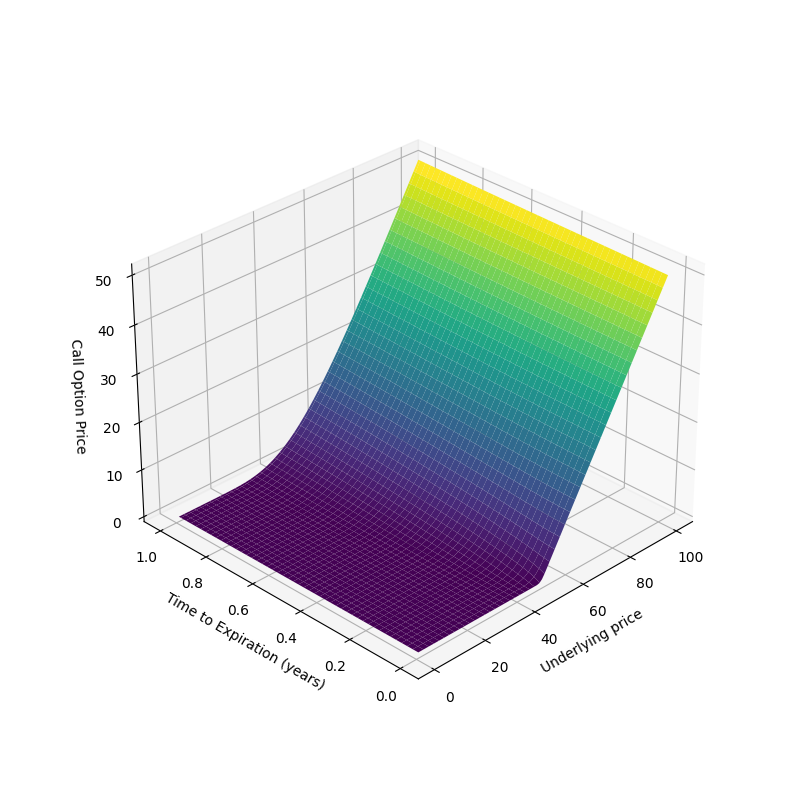
\includegraphics[width=1\textwidth]{pngs/direct.png}
		\caption{BS model pricing call option with parameters: \\
		strike = 50, rate = 2\%, volatility = 0.34}
	\end{figure}
	\begin{figure}[ht]
		\centering
		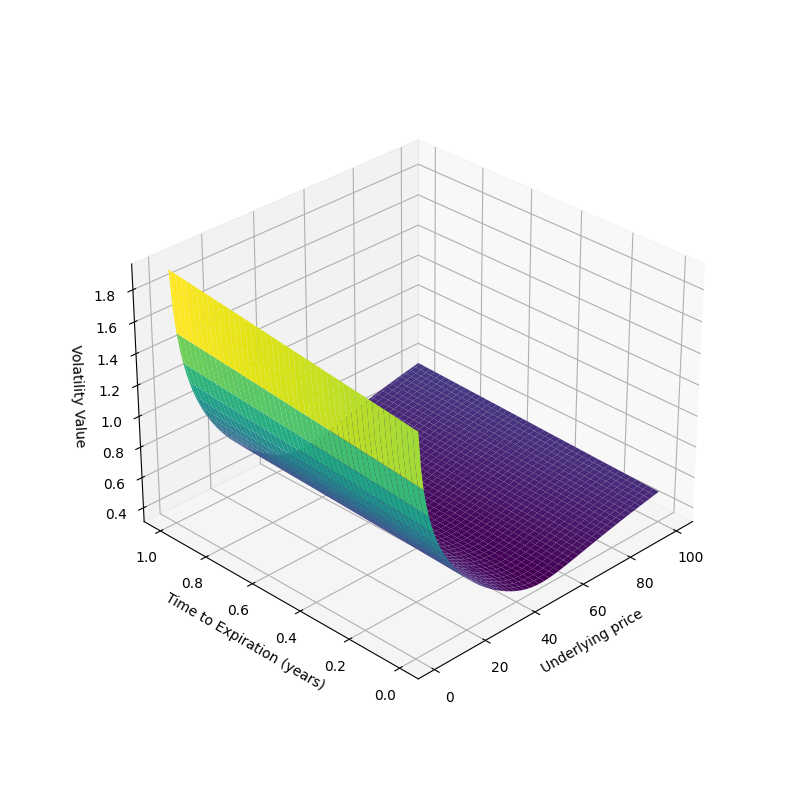
\includegraphics[width=1\textwidth]{pngs/volatility_surface.png}
		\caption{SABR volatility surface with parameters: \\
		strike = 50, rate = 2\%, $\alpha = 1.63, \beta = 0.6, \rho = -0.09, \nu = 1.3$}
	\end{figure}
	\begin{figure}[ht]
		\centering
		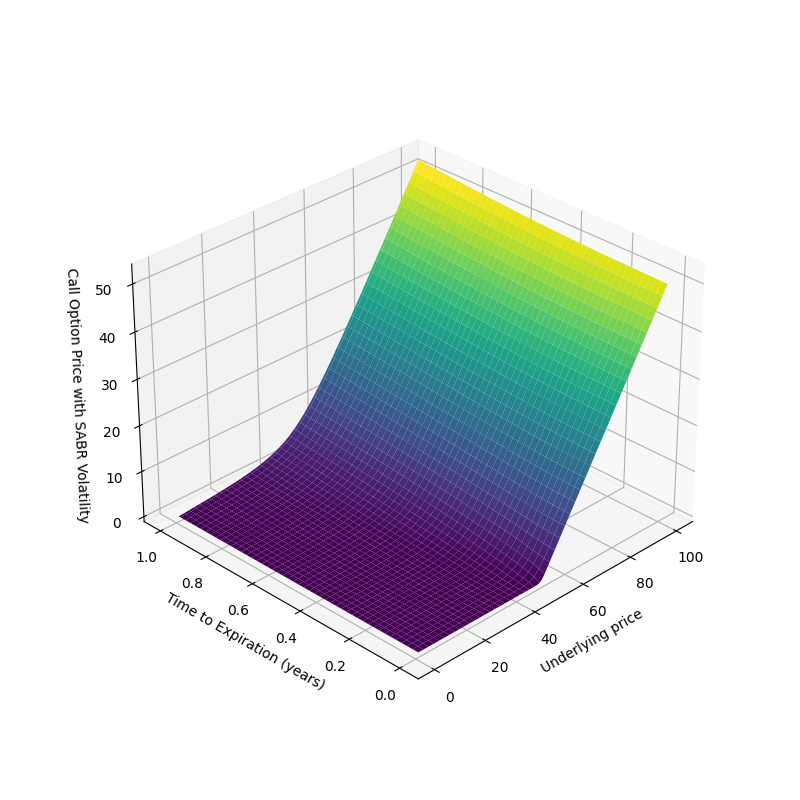
\includegraphics[width=1\textwidth]{pngs/bs_with_sabr.png}
		\caption{BS+SABR model price prediction with parameters: \\
		strike = 50, rate = 2\%, $\alpha = 1.63, \beta = 0.6, \rho = -0.09, \nu = 1.3$}
	\end{figure}
	\begin{figure}[ht]
		\centering
		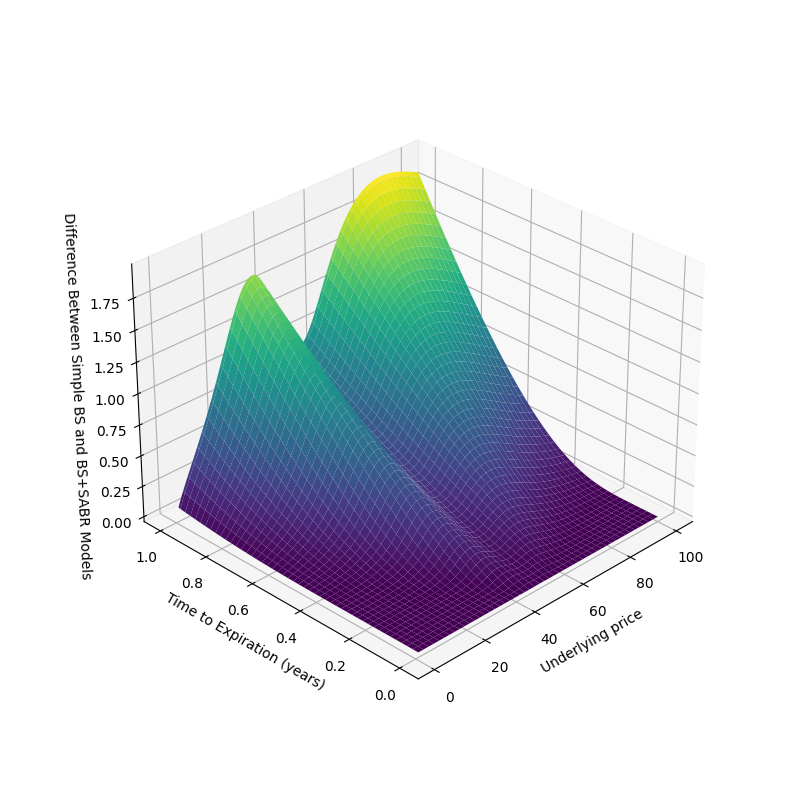
\includegraphics[width=1\textwidth]{pngs/bs_simple_vs_bs_sabr.png}
		\caption{Difference of two models}
	\end{figure}
	\begin{figure}[ht]
		\centering
		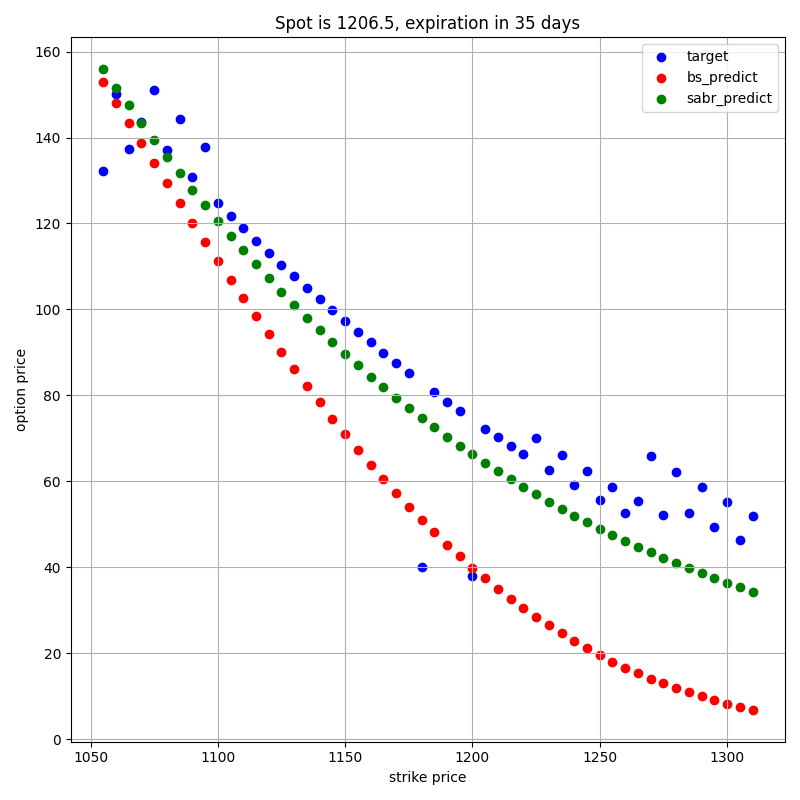
\includegraphics[width=1\textwidth]{pngs/2011-09-16-35.png}
		\caption{Comparing two models on a test part of real market data}
	\end{figure}
	\begin{figure}[ht]
		\centering
		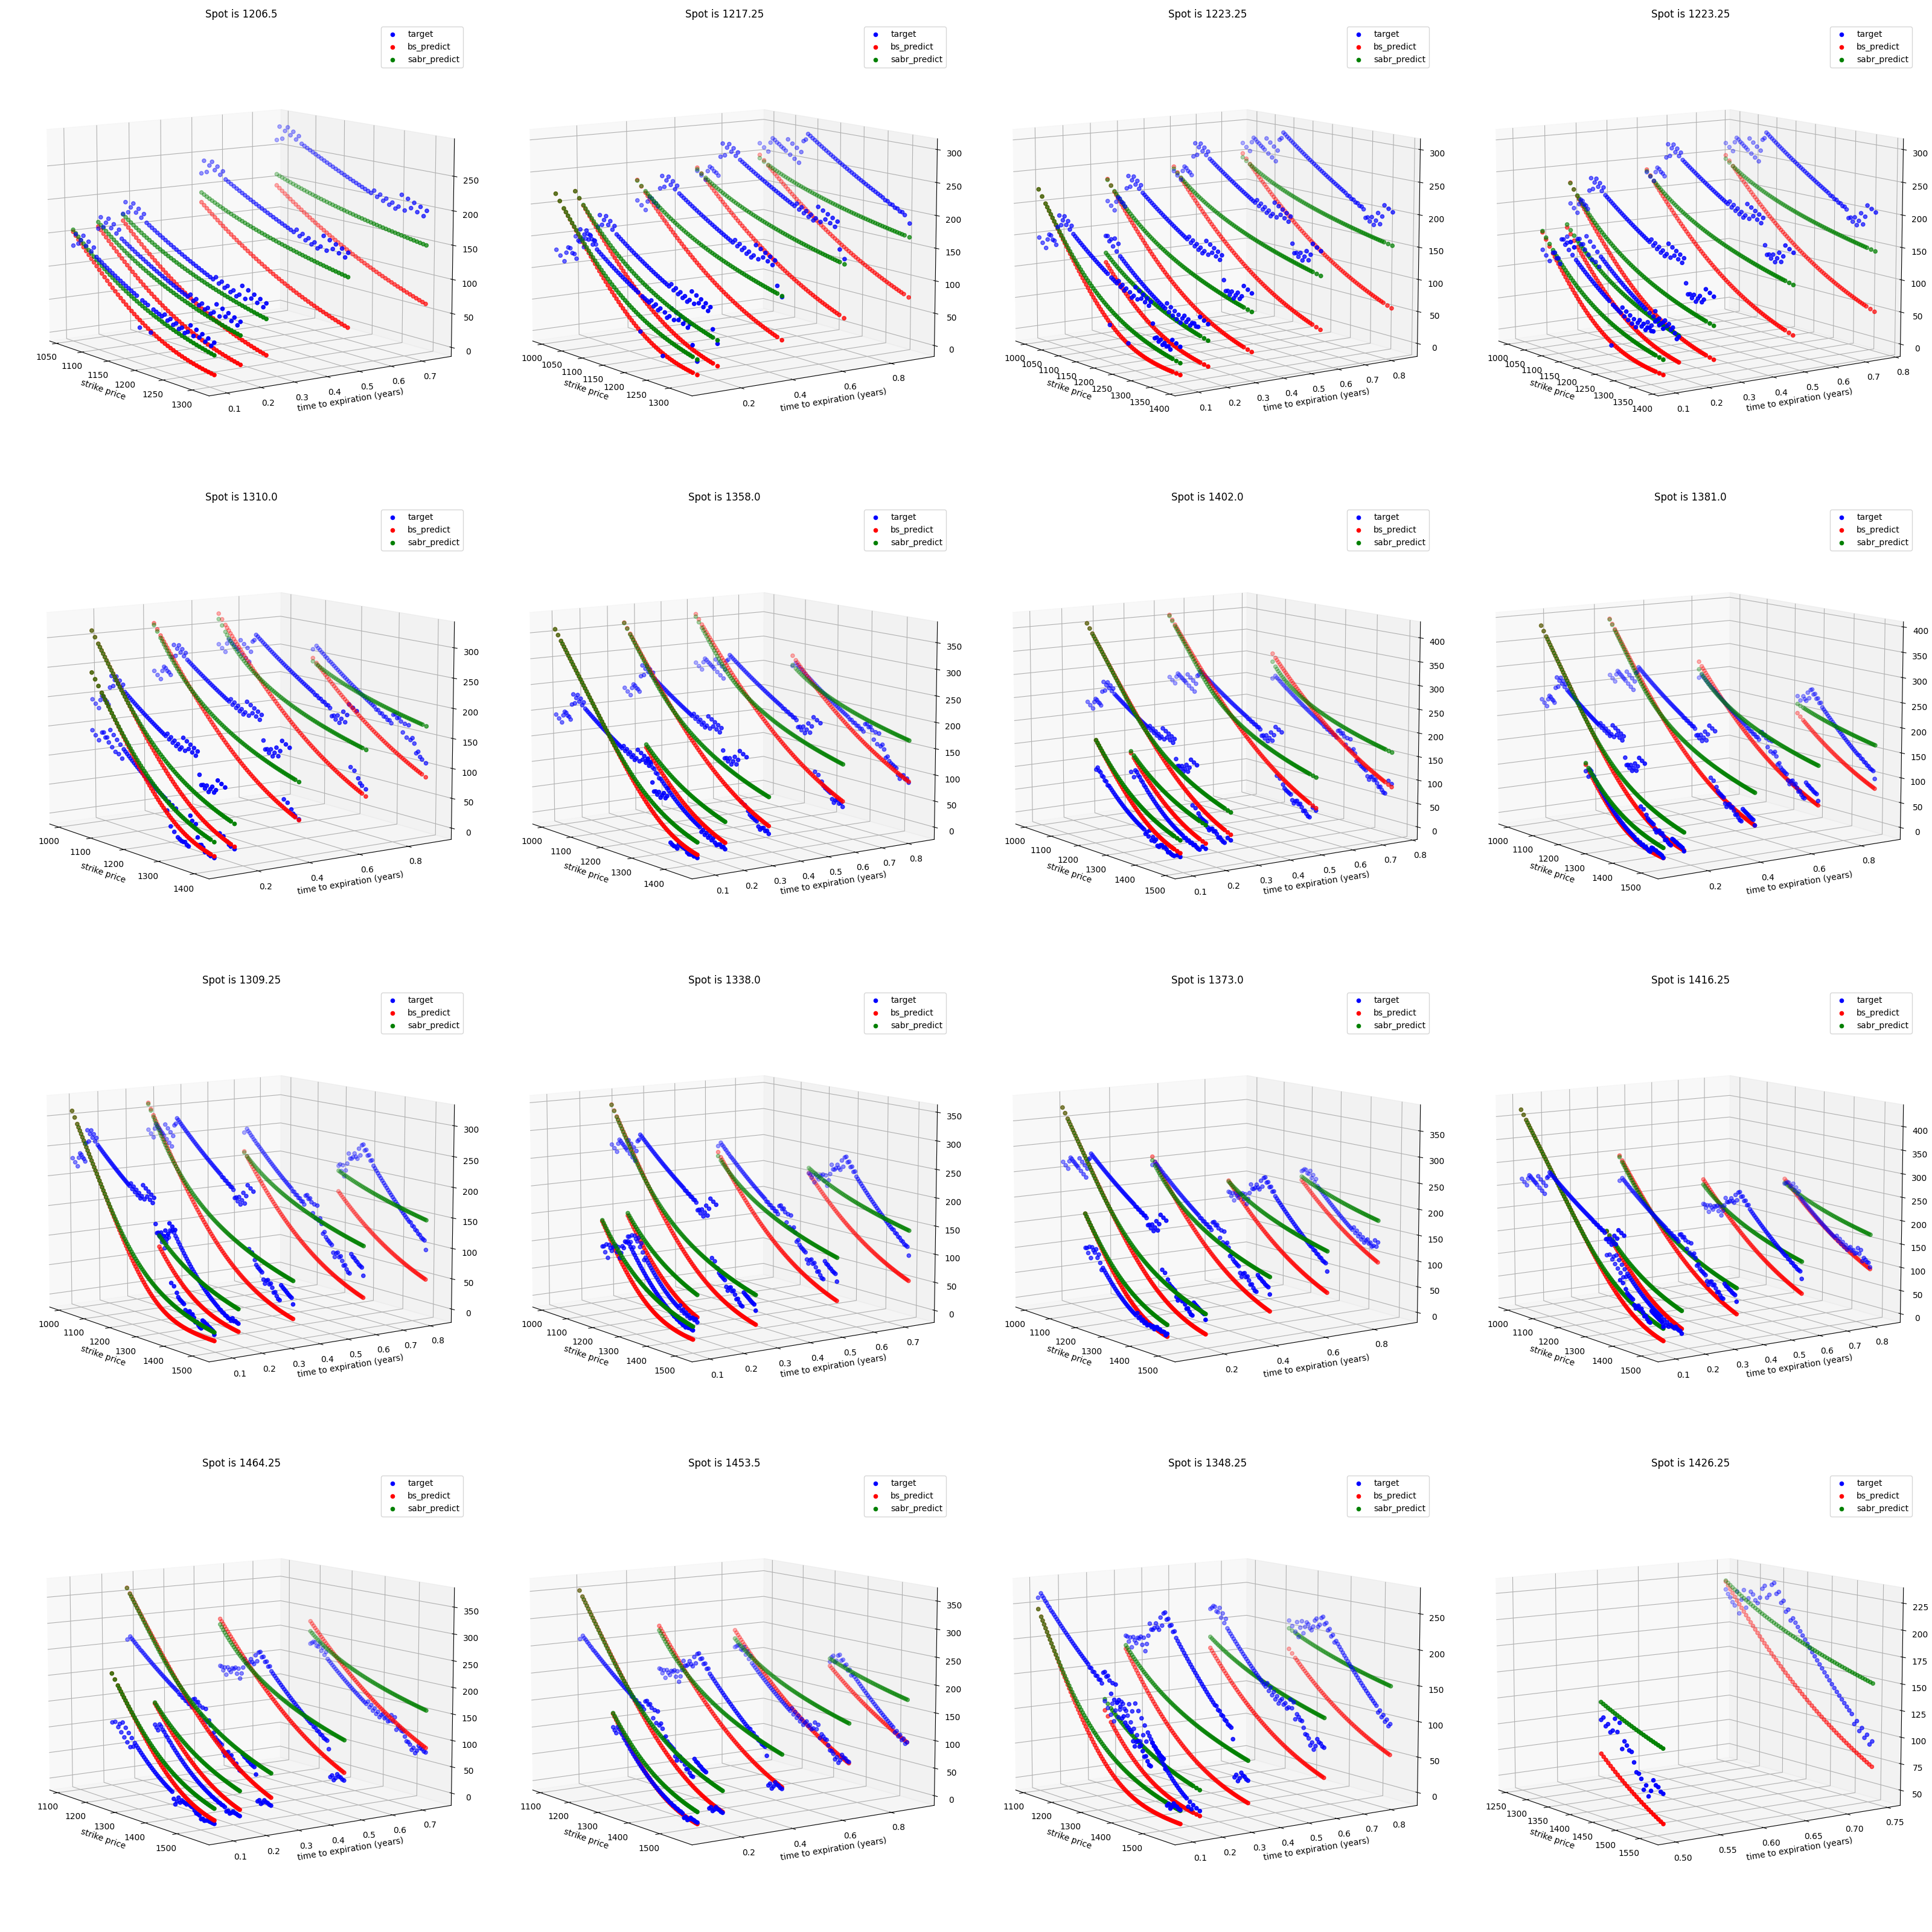
\includegraphics[width=1\textwidth]{pngs/summary.png}
		\caption{Summary of comparison}
	\end{figure}

\end{document}
